% Required packages: amsmath, amssymb, xcolor, tikz
% Required TikZ libraries: none
% Target width: 160 mm
% Minimum text size: 8 pt
% Colour/greyscale intent: one teal accent; direct labels preserve all distinctions
\begingroup
\definecolor{ealfigaccent}{RGB}{15,91,103}
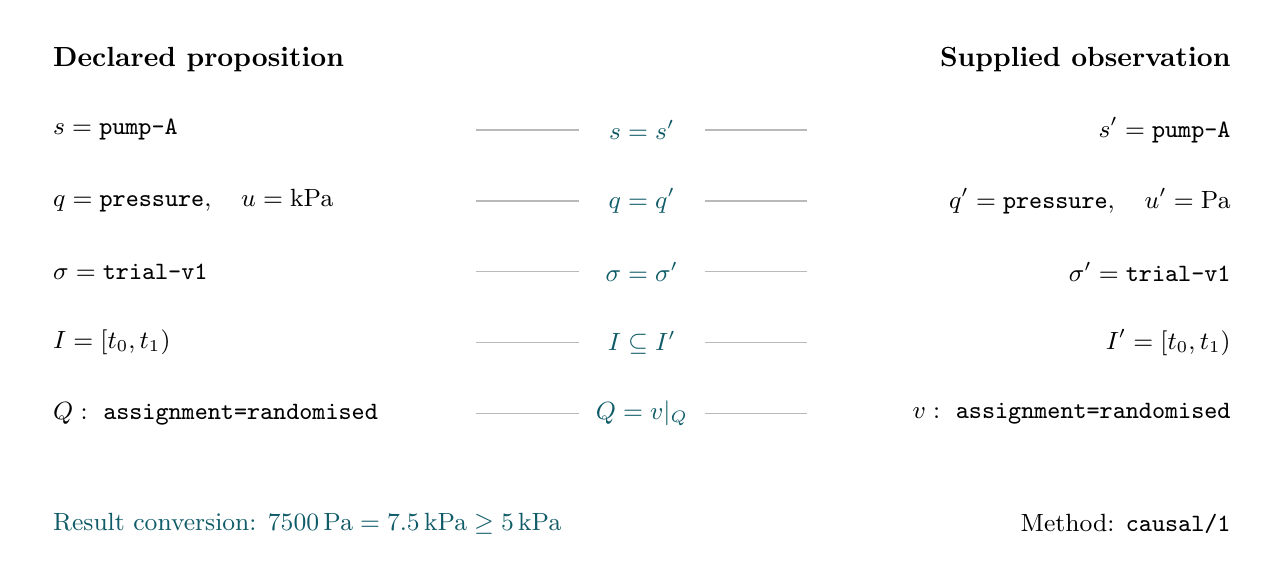
\begin{tikzpicture}[x=1mm,y=1mm,font=\fontsize{9}{11}\selectfont]
\path[use as bounding box] (0,0) rectangle (156,66);
\node[anchor=west,font=\bfseries] at (2,62) {Declared proposition};
\node[anchor=east,font=\bfseries] at (154,62) {Supplied observation};
\node[anchor=west] at (2,53) {$s=\texttt{pump-A}$};
\node[anchor=east] at (154,53) {$s'=\texttt{pump-A}$};
\node[anchor=west] at (2,44) {$q=\texttt{pressure},\quad u=\mathrm{kPa}$};
\node[anchor=east] at (154,44) {$q'=\texttt{pressure},\quad u'=\mathrm{Pa}$};
\node[anchor=west] at (2,35) {$\sigma=\texttt{trial-v1}$};
\node[anchor=east] at (154,35) {$\sigma'=\texttt{trial-v1}$};
\node[anchor=west] at (2,26) {$I=[t_0,t_1)$};
\node[anchor=east] at (154,26) {$I'=[t_0,t_1)$};
\node[anchor=west] at (2,17) {$Q:\ \texttt{assignment=randomised}$};
\node[anchor=east] at (154,17) {$v:\ \texttt{assignment=randomised}$};
\foreach \y in {53,44,35,26,17} {
  \draw[gray!55,line width=.45pt] (57,\y)--(70,\y);
  \draw[gray!55,line width=.45pt] (86,\y)--(99,\y);
}
\node[text=ealfigaccent] at (78,53) {$s=s'$};
\node[text=ealfigaccent] at (78,44) {$q=q'$};
\node[text=ealfigaccent] at (78,35) {$\sigma=\sigma'$};
\node[text=ealfigaccent] at (78,26) {$I\subseteq I'$};
\node[text=ealfigaccent] at (78,17) {$Q=v|_Q$};
\node[anchor=west,text=ealfigaccent] at (2,3) {Result conversion: $7500\,\mathrm{Pa}=7.5\,\mathrm{kPa}\geq5\,\mathrm{kPa}$};
\node[anchor=east] at (154,3) {Method: \texttt{causal/1}};
\end{tikzpicture}
\endgroup
